%% ------------- Portuguese version ------------
\documentclass{sbrt}
\usepackage[english,brazil]{babel}
\usepackage[utf8]{inputenc}
\usepackage{graphicx}
\newtheorem{theorem}{Teorema}
\usepackage{cite}
\usepackage{amsmath,amssymb,amsfonts}
\usepackage{algorithmic}
\usepackage{graphicx}
\usepackage{textcomp}
\usepackage{multirow}
\usepackage{url}
\usepackage[table, svgnames, dvipsnames]{xcolor}
\usepackage{eurosym}
\usepackage{soul}
\usepackage{subfig}
\usepackage{flushend}

\definecolor{green}{RGB}{11, 191, 60}

\newcommand{\hm}[1]{{\color{green}[HM] #1}}
\newcommand{\gled}[1]{{\color{red}[GS] #1}}

\newcommand{\todo}[1]{{\color{red}[TODO] #1}}
\newcommand{\rd}[1]{{\color{blue}[RD] #1}}
\newcommand{\pr}[1]{{\color{blue}[PR] #1}}


\begin{document}

\title{Aplicação de Internet das Coisas para o Monitoramento e Controle de Qualidade de Vacinas}

\author{Henrique M. Miranda, Gledson S. Souza, Ruan D. Gomes, Paulo Ribeiro Lins Júnior e Moacy P. Silva
\thanks{Henrique e Gledson são alunos do IFPB, Campus Campina Grande. Ruan, Paulo e Moacy são professores da Coordenação de Informática do IFPB -- Campina Grande. e-mails: henrique.miranda@academico.ifpb.edu.br, glegogle84@gmail.com, ruan.gomes@ifpb.edu.br, paulo.lins@ifpb.edu.br, moacy.silva@ifpb.edu.br. Esse trabalho foi financiado pelo IFPB e pelo CNPq.}
}

\maketitle

\markboth{XXXVIII SIMPÓSIO BRASILEIRO DE TELECOMUNICAÇÕES E PROCESSAMENTO DE SINAIS - SBrT 2020, 13--16 DE SETEMBRO DE 2020, FLORIANÓPOLIS, SC}{} 

\vspace{-2mm}
\begin{resumo}
O armazenamento é um dos componentes mais importantes da cadeia de distribuição de vacinas, principalmente pela sensibilidade delas a variações de temperatura, que podem ocasionar diminuição da sua eficácia. Considerando isso, existe uma necessidade de manter constante monitoramento dessa variável, afim de garantir que o produto final venha a manter suas característica originais e a eficiência esperada. Esse trabalho apresenta uma solução baseada em Internet das Coisas, usando comunicação sem fio de baixa potência, para monitorar a qualidade de vacinas, por meio das medidas de temperatura e umidade nos locais de armazenamento. Os dados coletados são organizados em um banco de dados, podendo ser acessados por sistemas decisórios afim de avaliar a qualidade da vacina antes de sua aplicação, evitando problemas em decorrência de problemas de armazenamento. %\pr{(aqui tem 127 palavras...não sei o limite do resumo).}

%Vacinas devem receber uma atenção especial com relação à maneira de armazenamento, visto que elas são sensíveis a alterações de temperatura e, consequentemente, podem perder a efetividade se submetidas a condições inadequadas. Desse modo, deve-se armazena-las em locais adequados e, idealmente, realizar um monitoramento em tempo real. Nesse contexto, este artigo descreve uma solução baseada em Internet das Coisas, para coletar dados de temperatura e umidade em locais de armazenamento de vacinas. Esses dados são armazenados em um banco de dados, de modo que as informações podem ser acessadas a qualquer momento. Além disso, é possível gerar notificações quando os parâmetros monitorados estão fora dos padrões corretos de conservação. , que pode ser realizado por meio de um aplicativo \textit{mobile}.

\end{resumo}
\begin{chave}
    Monitoramento, vacinas, IoT, LoRa. 
\end{chave}
%% ---------------------------------------------

%\begin{abstract}
%    Vaccines should have special attention on the stored, since, they are susceptible to temperature changes and, consequently, loss of qualities, reducing your efficiency. Therefore, special care must be taken, not only in the correct storage location but on your monitoring that way that can be accompanied on real-time.

%\end{abstract}
%\begin{keywords}
%    Vaccines, Temperature, Humidity, Quality.
%\end{keywords}
\chapter[Introdução]{Introdução}
\label{cap:intro}
% ---

A saúde é um fator de suma importância para todos os seres vivos, ele é um problema científico, tecnológico, político, prático e filosófico que refere-se a um estado completo de bem estar físico, emocional, social, intelectual e espiritual \cite{almeida2011saude}. 

Segundo o artigo 196 \cite{de2013direito} da Constituição Federal Brasileira a saúde é um direito de todos e dever do Estado garantir medidas políticas sociais e econômicas que visam à diminuição do risco de doenças e de outros agravamentos e ao acesso universal e imparcial às ações e serviços para a sua promoção, proteção e recuperação.

Para garantirmos nossa saúde, precisamos cuidar do nosso corpo e mente, para isto, uma ferramenta que podemos contar são os imunobiológicos, como as vacinas e os soros, diferente de remédios que ajudam no tratamento de pessoas doentes, as imunobiológicos são uma preparação biológica que fornece imunidade total ou parcial de uma determinada doença autoimune para um indivíduo saudável. As vacinas e os soros se diferem pela sua forma de imunização, as vacinas fornece uma imunização ativa, estimulando o nosso organismo na produção de anticorpos, os soros fornecem uma imunização passiva, provendo os anticorpos para o nosso organismo que foram produzidos  em outros organismo \cite{soma2018tratamento}.

Contudo, os imunobiológicos requerem um cuidado elevado para manter a qualidade e sua eficiência, um dos fatores é que são produtos termolábeis, ou seja, se deterioram após determinado tempo expostos a variações de temperaturas e umidade, portanto, é imprescindível assegurar que seu ambiente de armazenagem mantenha uma temperatura e umidade consante \cite{ministerio2001manual} para garantir uma longevidade maior para o produto. Para este propósito, existem as redes de frio, um processo desenvolvido pelo Programa Nacional de Imunizações, PNI, de conversação, armazenamento e transporte dos medicamentos, objetivando as condições adequadas dos mesmos, mantendo suas características iniciais \cite{ministerio2001manual}.

No ano de 2014, foi relatado em um estudo \cite{oliveira2014avaliaccao} que a qualidade de conservação das vacinas não eram adequadas em boa parte dos municípios da macroregião Oeste de Minas Gerais, alguns dos motivos citados foram a má gestão dos refrigeradores, falhas no minitoramento da temperatura e insuficiência de recusos humanos.



\begin{itemize}
  \item \todo{Falar sobre dificuldade no controle de qualidade}
  \item \todo{Falar da IoT}
  \item \todo{Falar da solução proposta}
\end{itemize}

\section{O Programa Nacional de Imunizações}
\label{intro:justificativa}

Com o sucesso da Campanha de Erradicação da Varíola, CEV, iniciada em 1965, tendo seu fim em 1973 \cite{muniz2011memorias}, amplificou dentro do Ministério da Saúde maiores investimento no controle de doenças autoimune, dando um impulso na criação do PNI \cite{temporao2003programa}. O PNI foi fundado com objetivo de controlar e erradicar as doenças imunopreveníveis, através de ações metalizadas de vacinação da população. Em 1980 foi realizada a primeira campanha de vacinação da poliomielite e desde então foram realizadas diversas campanhas, tais como a da rubéola, sarampo, tuberculose febre amarela entre outras \cite{temporao2003programa,ministerio2001manual}.

De acordo com a Lei n.º 6.259 de 30 de outubro de 1975, regularizada pelo Decreto nº 78.231 em 1976, certificar o PNI, sobre a responsabilidade do Ministerio da Sáude e define as seguintes competências \cite{ministerio2001manual}:
  \begin{itemize}
    \item implantar e implementar as ações do Programa, relacionadas com as vacinações de caráter obrigatório;
    \item  estabelecer critérios e prestar apoio técnico e financeiro à elaboração, implantação e implementação dos programas de vacinação a cargo das secretarias de saúde das unidades federadas;
    \item estabelecer normas básicas para a execução das vacinações;
    \item supervisionar, controlar e avaliar a execução das vacinações no território nacional, principalmente o desempenho dos órgãos das Secretarias de Saúde, encarregados dos programas de vacinação.
  \end{itemize}
% ---
\section{Justificativa e Relevância do Trabalho}
\label{intro:justificativa}



\begin{itemize}
  \item \todo{Falar das perdas e prejuizos}
  \item \todo{Falar dos beneficios ao usar um aplicão desse porte}
\end{itemize}

% ---
\section{Objetivos}
\label{intro:objetivos}

\subsection{Objetivo Geral}
\label{intro:objetivos:geral}
Construir uma arquitetura baseada em conceitos de IoT visando o monitoramento de temperatura e umidade de imunobiológicos para auxiliar funcionários da saúde, garantindo melhores condições para a vacinação da população frente a incidência de doenças.

\subsection{Objetivos Específicos}
\label{intro:objetivos:especificos}
\begin{itemize}
  \item Construir um protótipo inicial para coleta da temperatura e umidade nos ambientes de armazenagens dos imunobiológicos.
  \item Implementar um servidor para a armazenagem dos dados coletados e posteriormente fornecer históricos das temperaturas e umidade ao aplicativo móvel.
  \item Desenvolver um aplicativo móvel para fornecer uma interface amigável para os usuários auxiliando no controle de qualidade dos produtos.
  \item Realizar testes e análises dos dados de transmissões a fim de garantir a confiabilidade das temperaturas e umidade coletadas.
\end{itemize}

% ---
\section{Metodologia}
\label{intro:metodologia}
No intuito de alcançar os objetivos pretendidos, a metodologia utilizada neste trabalho
foi composta pelas seguintes etapas:

\begin{itemize}
  \item \todo{Adicionar os pontos}.
\end{itemize}

% ---
\section{Organização do Documento}
\label{intro:organizacao}
\hm{A ser feito quando o documento tiver pronto}
\section{Descrição do Sistema}
    %\gled{O projeto é dividido em "nós" que ficam encarregados de obter os dados da aplicação e enviar para um gateway responsável por capturar os dados e enviar para um servidos, para ter a disposição todos os dados com seu conteúdo obtido e confirmação se o pacote foi entregue com sucesso. }
    
    Objetivando a garantia de disponibilidade do sistema, optou-se pelo uso de um sistema de comunicação sem fio de baixo consumo de energia, utilizando a tecnologia LoRa e o protocolo de comunicação LoRaWAN, que permite ao sistema comunicação de longo alcance com baixo consumo energético.
    
    O sistema (Figura \ref{fig:arch}) é composto por nós finais, um \textit{gateway} e um servidor, além de aplicações cliente, para acesso aos dados e recebimento das mensagens de alarme. As partes são detalhadas nas subseções a seguir.
\begin{figure}[t!]
    \begin{center}
        \centering
        %\setlength{\unitlength}{0.0050in}
        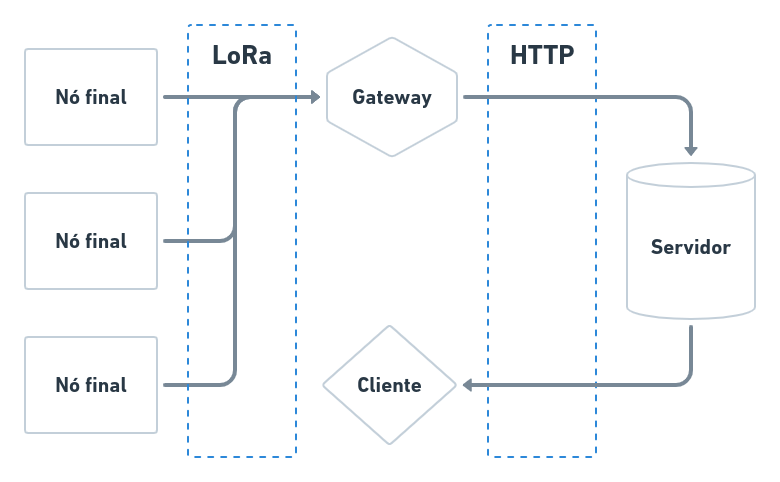
\includegraphics[width=0.4\textwidth]{assets/schematic.png}
    \end{center}
    \caption{\label{esquema} Arquitetura geral do sistema.}
    \label{fig:arch}
\end{figure}
%\subsection{Nó Final}

    Os nós finais são utilizados para obter dados coletados pelos sensores de temperatura e umidade e transmiti-los para um \textit{gateway}, por meio de  um transceptor LoRa \cite{ref2}. O fator de espalhamento (SF) do LoRa, que vai de 6 até 12\cite{ref3}, define a taxa de bits. Foi utilizado nos testes o SF igual a 7, que é o valor padrão da biblioteca usada \cite{ref4}. As camadas superiores podem ser implementadas seguindo o padrão aberto LoRaWAN entre os nós finais e o \textit{gateway}. O LoRa pode trabalhar, nas Américas, na faixa de 915~MHz \cite{ref2}. % a 928~Mhz.%, no nosso caso, optamos por usar 915~Mhz.
    
    Os nós finais utilizam o sensor DHT22 \cite{ref6} para a captação dos dados dos ambientes de armazenagem, podendo medir temperaturas entre -40$^\circ$C a 80$^\circ$C, com precisão em torno de $\pm$ 0,5$^\circ$C, e umidade de 0 a 100\%, com precisão de 0,1\%.

    O \textit{gateway} é formado por um microcontrolador com uma interface LoRa e uma interface Wi-Fi, para comunicação com os nós finais e conexão com a Internet, respectivamente. Quando ativado, ele cria um \textit{access point}, de modo que é possível se conectar para mudar as configurações de rede, se necessário, e tenta se conectar a uma rede Wi-Fi pré-configurada. Com êxito, ele recebe os dados dos nós finais, realiza a detecção de  erros  de  formato  no  pacote,  e  transmite  os  dados  para um  servidor  na  nuvem.  Essa  transmissão  para  o  servidor  é realizada através de requisições HTTP.
    
   %\rd{(O que foi usado para implementar o gateway? Como ocorre a conexão com a internet?.)}
    O servidor é responsável por armazenar os dados dos usuários, como e-mail e senha, dados dos nós finais e do \textit{gateway}, tais como identificadores e localização, além dos dados coletados pelos sensores, junto com os dados dos pacotes transmitidos pelos nós finais, como o RSSI, essencial para a realização dos testes, pois podemos analisar a qualidade dos enlaces de comunicação.
    
    O cliente é um aplicativo para Android responsável por exibir os dados coletados pelos nós finais cadastrados entre outras funções.
    %, além de permitir criar, editar e deletar os dados dos nós e dos \textit{gateways}.
\section{Avaliação do Sistema}
   
   A Figura~\ref{fig:prot} mostra os protótipos desenvolvidos para testes iniciais com o sistema (nó final do lado esquerdo e \textit{gateway} do lado direito). Após uma sessão de testes, foi possível avaliar no experimento a eficiência de transmissão e recepção de dados.%, bem como o consumo de energia do nó final.% levando em consideração as possíveis variáveis que impedem a realização de testes.
   
   \begin{figure}[t!]
    \begin{center}
        \centering
        %\setlength{\unitlength}{0.0105in}
        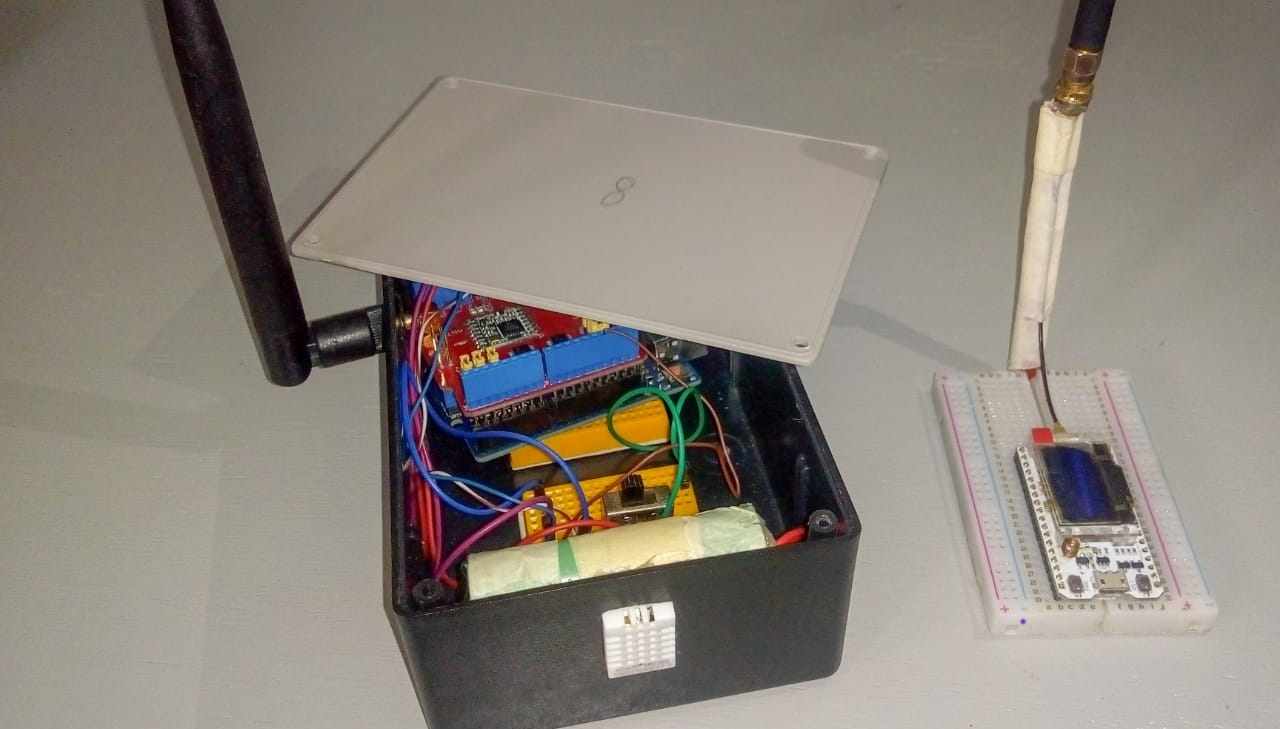
\includegraphics[width=0.4\textwidth]{assets/prototipo.jpeg}
    \end{center}
    \caption{Protótipos desenvolvidos para a realização dos testes.}
    \label{fig:prot}
\end{figure}
   
   Os experimentos foram realizados no bloco dos professores do IFPB--Campus Campina Grande \cite{ref7}. O \textit{gateway} foi posicionado em um espaço, no térreo, enquanto que o transmissor foi posicionado em outro espaço, no sub-solo, distando aproximadamente  60 metros um do outro, e contando com vários obstáculos à comunicação, como paredes densas, laje, objetos metálicos e equipamentos eletrônicos.
   
  O gráfico na Figura~\ref{fig:pdrrssi} apresenta a Taxa de Entrega de Pacote (PDR) a cada hora, em um teste com duração de 24 horas, em que o nó final realizou envios contínuos de pacotes em intervalos de 5 minutos. A PDR geral foi de 78.82\%, no entanto, em alguns momentos a PDR ficou em torno de 20\%, o que pode ter sido ocasionado por modificações no perfil de multi-percurso do ambiente, obstáculos temporários ou presença de fontes de interferência. Considerando a taxa de transmissão de pacote utilizada, com PDR de 20\% ainda é possível obter uma nova informação a cada 25 minutos, em média, o que é suficiente para a realização do monitoramento de temperatura e umidade, que são grandezas que variam lentamente. No entanto, os resultados ressaltam a importância de se desenvolver estratégias para aumento de confiabilidade na transmissão de pacotes de alerta. Pode-se empregar, por exemplo, estratégias de redundância, como replicação de pacote, diversidade de frequência ou de modulação. Essas possibilidades serão estudadas em trabalhos futuros.
   %para permitir um aumento de confiabilidade do sistema.
   
   A Figura~\ref{fig:pdrrssi} também mostra o RSSI médio e o desvio padrão. No protótipo foi utilizado um transceptor  RF96, que pode operar com uma sensibilidade superior a -148dBm [5]. A potência utilizada na transmissão de dados foi  de 17~dBm, que é a potência padrão utilizada na biblioteca do LoRa.%\rd{(precisa saber a sensibilidade do transceptor, para uma discussão melhor. Outra informação importante que faltou foi a potência de transmissão usada.)}
   
    % -------------------- dados legais -------------------- 
    % Potência de transmissão usada:  
    % - +17dBm (a padrão da lib do Arduíno **Lora by Sandeep Mistry** usada)
    % - pode ser configurado +2dBm até +20dBm
   
    % Sensibilidade do transceptor (Tirado do datasheet [3]):
    % - Dynamic Range RSSI -> 127 dB
    % Using Semtech’s patented LoRaTM modulation technique
    % SX1276/77/78/79 can achieve a sensitivity of over -148dBm
    % using a low cost crystal and bill of materials. The high
    % sensitivity combined with the integrated +20 dBm power
    % amplifier yields industry leading link budget making it
    % optimal for any application requiring range or robustness. 
   
   
   \begin{figure}[t!]
        \begin{center}
            \centering
            \setlength{\unitlength}{0.0105in}
            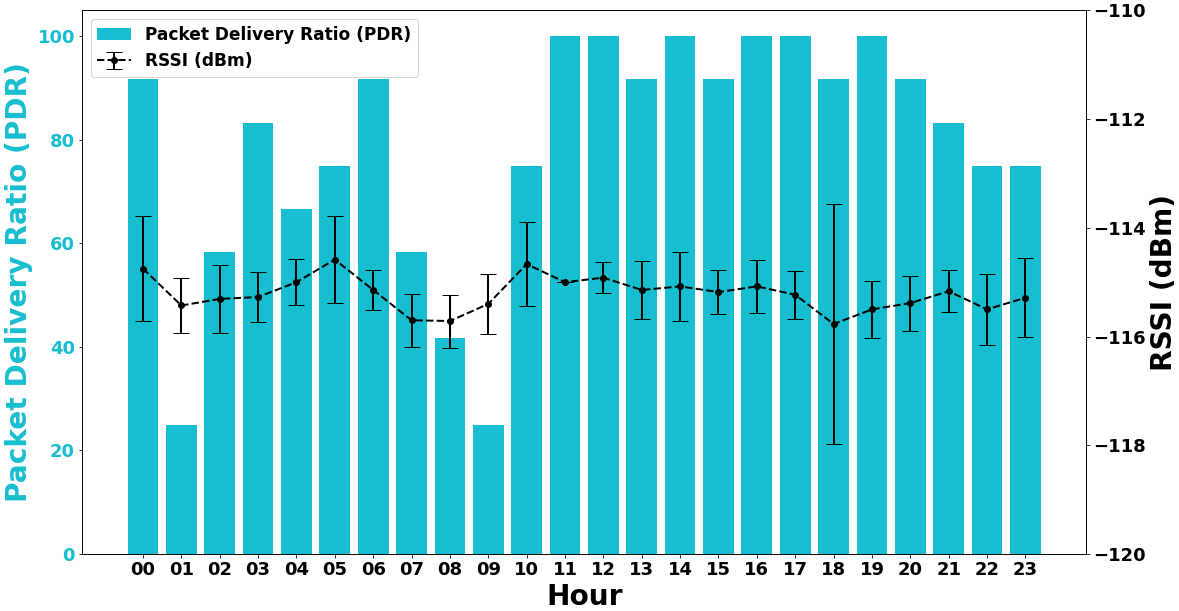
\includegraphics[width=.45\textwidth]{assets/pdr-rssi-5.png}
        \end{center}
        \caption{Percentual em entrega dos pacotes em barras e indicador de intensidade do sinal recebido em linha.}
        \label{fig:pdrrssi}
    \end{figure}
\chapter{Considerações Finais}
\label{cap:conlusao}


\section{Sugestões para Trabalhos Futuros}
\label{sec:futuros}
%\section*{Agradecimentos}
    Agradecemos aos laboratórios Assert e GcomPI, do IFPB, e ao CNPq.% do IFPB-CG e todos os professores envolvidos, que nos ajudaram e nos apoiaram fornecendo o espaço para o desenvolvimento do projeto.
\begin{thebibliography}{99}

    \bibitem{ref7} Autoral. Repositorio do Github com os testes realizados.  Disponível em: https://github.com/GComPI-IFPB/lora-transmitter-test. Acessado em 22 de maio, 2020.
    
    \bibitem{ref1} Ministerio da Saude. Manual de Rede de Frio.  Disponível em: http://bvsms.saude.gov.br/bvs/publicacoes/manual\_rede\_frio4ed.pdf. Acessado em 13 de abril, 2020.
    
    \bibitem{ref2} LoRa Alliance. Regional Parameters. Disponível em: https://lora-alliance.org/sites/default/files/2020-01/rp\_2-1.0.0\_final\_release.pdf. Acessado em 15 de abril, 2020.
    
    \bibitem{ref3} Semtech Corporation. Datasheet SX1276/77/78/79. Disponível em: https://www.curtocircuito.com.br/datasheet/modulo/SX1276.pdf. Acessado em 24 de abril, 2020.
    
    \bibitem{ref4} Sandeep Mistry. Documentação da biblioteca LoRa utilizada para Arduíno. Disponível em: https://github.com/sandeepmistry/arduino-LoRa. Acessado em 11 de maio, 2020.
    
    \bibitem{ref5} Universidade Estadual Paulista. Técnicas de Múltiplo Acesso para Redes LORAWAN. Disponível em: https://repositorio.unesp.br/bitstream/handle/11449/156791/000902295.pdf. Acessado em 11 de maio, 2020.
    
   \bibitem{ref6} Thomas Liu. Datasheet DHT22. Disponível em:  https://www.alldatasheet.com/datasheet-pdf/pdf/1132459/ETC2/DHT22.html. Acessado em 18 de maio de 2020.
    
\end{thebibliography}

%\appendix
%Aqui vão informações mais apropriadas para um apêndice.

\end{document}
